\documentclass{article}
\usepackage{inputenc}
\emergencystretch=2em
\usepackage[breaklinks]{hyperref}
\hypersetup{
    colorlinks=true,
    linkcolor=blue,
    filecolor=magenta,      
    urlcolor=magenta,
    citecolor=black}
    
\usepackage[english]{babel}
\usepackage{biblatex}
\usepackage{svg}
\usepackage{graphicx}
% For line numbers
\usepackage[left]{lineno}


%%%% For the scheme
%\usepackage{tikz}
%\usetikzlibrary{matrix,shapes}
%\setlength{\parindent}{0pt}
%\usepackage{pgfgantt}
%\usepackage{lscape}

%%% For the thesis rings %%%
%\renewcommand{\baselinestretch}{2.0}
%
\linenumbers


\addbibresource{references.bib}
\title{A Step Towards Explained AI: Creating a Semantically Clean Database for Infering Species with Natural Language} 

%Explainable Artificial Intelligence: Using Natural Language as Intermediate Result Between Two Deep Learning Models}
\author{Robert Vlasakker, van de}
\date{August 2021}

\begin{document}
\graphicspath{ {./figures/} }

\maketitle

\section{Introduction}
Deep learning allows for incredible applications from the automatic classification of text and images, natural language processing to reinforcement learning.
In many cases, especially in the case of computer vision, deep learning models have already surpassed human experts \cite{he_delving_2015}.
Because of their success, deep learning vision models are already found quite often in consumer-grade electronics, like smartphones and used in a lot of different application like the \href{https://www.inaturalist.org/}{iNaturalist} application.
%With the \href{https://www.inaturalist.org/}{iNaturalist} model, species can automatically be recognized just by taking a picture of species \cite{radford_learning_2021}.
In natural language processing (NLP), auto-regressive models like GPT-3 (Generative Pre-trained Transformer 3) can produce text that barely can be distinguished from a text produced by real humans \cite{brown_language_2020}.
Microsoft even acquired an exclusive licensing on GPT-3 on 22 September 2020 and will integrate the model into their products and services.
While these results and their applications of the deep learning models are incredible, the reasoning behind the results remains a mystery in most cases \cite{li_interpretable_2021, losch_interpretability_2019}.

Unlike classic machine learning models, deep learning models can automatically extract features needed for detection or classification.
Domain knowledge, in combination with careful engineering to extract the necessary features for the detection and/or classification, is no longer needed \cite{lecun_deep_2015}.
While this automatic feature extraction is very convenient, it reduces the interpretability of the models.
To extract the features of the input data, deep learning models use multiple simple neurons that take the input, process it to a slightly more abstract representation and pass it through the next neuron.
Provided enough neurons are 'stacked' upon each other, very complex features can be extracted and correctly detected and/or classified by such a network.
At passing the data also becomes a bit more abstract and less interpretable.
Stacking multiple neurons on top of each often results in millions of parameters in most recent deep learning models (or even billions in the case of GPT-3).
All of these neurons use  non-linear activation functions that increase the overall complexity of the network.
These parameters are the coefficients of the model
They are initially chosen by the designer or randomly initialized by the model and get updated by the model as it 'learns'\footnote{The learning method varies across different deep learning models, but is based on derivatives.} from the data.
After training, the parameters of the model can no longer easily interpreted.
This behaviour is often referred to as a 'back box', which means that the reasoning behind the result is tough to understand or is lacking at all.
The increasing complexity already resulted in several regulations, where the European General Data Protection Regulation (GDPR) is maybe the most famous one.
With sensitive fields, like health care, financial classification or autonomous driving, this black box behaviour could raise issues as it hampers the trustworthiness of the models. \cite{carvalho_machine_2019}.
In these fields it is very important to keep the models comprehensible for humans as the decision of a model will have an impact on human lives.
Also when the reasoning behind deep learning behaviour is better understood, the insights could also lead to the improvements of these models \cite{amershi_modeltracker_2015} and deep learning models can be expanded to more fields \cite{lei_opening_2018}.
Different algorithms and techniques have been proposed to increase the interpretation of the models, like feature reduction algorithms \cite{ribeiro_why_2016}, inference of training sample contribution \cite{koh_understanding_2020} or by changing jittering test samples and see how the prediction changes \cite{li_understanding_2017}.
%One of the most popular techniques for making deep learning models easier to interpret are decomposition and partial derivatives techniques \cite{samek_explainable_2017}.
%Both techniques use heat maps.
%The heat map of a decomposed model will show how much each pixel contributes to the model's prediction.
%The heat map of a model with partial derivatives will show how much the changes in each pixel affect the model's prediction.
Van Lent et al. already coined the term explained artificial intelligence (XAI) in 2004 as the ability to explain behaviour of AI in game applications. \cite{van_lent_explainable_2004}.
While some advances have been made in model understanding, large leaps forward in the field of XAI remain limited \cite{lipton_mythos_2017, li_interpretable_2021}.

In the taxonomy, new species are described now by experts in the field.
Estimated is that 50\% of the species are yet to be discovered, and many species will go extinct before every described.
Scalable technologies that can help monitor diversity and help discover new species are more needed than ever.
Deep learning models can help discover new species, automate and speed up this process.
It is, however, important to better understand the reasoning of a deep learning model in such a sensitive case \cite{carvalho_machine_2019}, why are certain species labelled as new and others are not?
XAI is very important is the field of taxonomy; it is very important to 'teach' deep learning models how taxonomy experts describe new species and in the meantime keep the model output interpretable for humans.
This way reasoning of the model can be tracked, evaluated and improved.
A regular classification model will predict a species based on what it sees on an image, and can then match this prediction against a known database.
While recent deep learning model vision model give amazing results with images with a known label, it is vital to see how the model's reasoning works in the case of newly predicted species.
Based on what parts of the image (e.g. color, pattern, parts) does the model classify species on an image as undiscovered.
By splitting this basic vision model, into a zero-shot vision model and a NLP model this problem might be solved and create a more explainable AI.
The first model will take an input image and instead of directly predicting a species, its output will be data in natural language about what it 'sees' (e.g., "3-petal with a pink color.", "The bill is black with blue spots.").
The second model will be a pure NLP model.
This model will take the prediction without any information about the species from the first model and tell which (new) species it predicts.
For both models a large database with species description is needed. 
This dataset needs either as many unique description sentences as possible for each species.
The other option is to process the language data into a more semantic database like a knowledge graph \cite{ontotext_what_2021}.
This research will focus on the first part the generation of a database that contains species names and their descriptions.
Second, it will focus on the species name generation based on on description data. 
These descriptions will be generated by a zero-shot vision model that is part of another research.


\section{Objective}
The first objective of this research is to create a large database with species names and their corresponding descriptions. 
There should not be any double species name in this database. 
If the species description is not available the descriptions will be stored per genus or family. 
%The descriptions should consists of single sentences and semantically there should not be any double sentences about the same species. 
The database could either contain unique sentences per species. 
In this case as many sentences per species have to be obtained.
An other approach is to extract the object/subject relations and store all information in a knowledge graph.
With this approach object/relation/subject (triples) will be extracted from the data. 
The root node will be the species.
\newline
\newline
\noindent  
\emph{How can a high quality database be created that contains species names and contains a combination of semantically unique descriptions per species, without revealing the name of the species in their corresponding descriptions.}
\noindent    
\newline
\newline
The second objective will be the creation of a NLP model that can infer species names based on description data. 
The data that will be fed to the model will consist of species description data that 
This could either be a existing species or the model could suggest a new species. 
It should be tractable which description sentences are important for inferring a certain (new) species. 
This is why two different databases are tested, either direct sentences or the sentences processed into a knowledge graph.
\newline
\newline
\noindent  
\emph{How should a deep learning model be built and trained to predict existing species from the used database and predict new species that do not, while in the meantime keep it possible to track of the most important keywords used for the prediction?}

\section{Approach}
%Transferlearning
% The first is a visual-language hybrid model that takes an image as input and generates descriptions of the image in natural language using the vocabulary of expert taxonomists, but is not aware of species names.
\subsection{Creation of the Dataset}
The first is to create a database that contains species names and their descriptions.
The World Wide Web has potentially and endless amount of species and species descriptions available.
However, this data is not structured and is certainly not in one place on the internet.
A webclawler that can automatically query species description pages from search engines and then search those queried pages for description sentences is the best to fill a large data base with species names and descriptions. 
A few consideration should be made:
Description sentences can be theoretically limitless, e.g. for a Brown Bear description sentences could be: 'The fur is brown.', 'The brown bear has brown fur.'.
Sentences can also have a more difficult semantic, e.g. 'The fur of the Brown bear is similar to that of the Grizzly bear'.
In previous cases it will not be feasible to use a classic machine learning approach that requires a rule-based system for the feature extraction from the data before classification. 
A deep learning model that can automatically extract the features and classify the text is needed in this case.
However, to properly train a deep learning model that is able to classify text data, a large, accurate and consistent labeled dataset is needed \cite{munappy_data_2019}.
For the creation of this dataset, several structured web sources like \href{http://www.Wikipedia.com}{Wikipedia}, \href{https://birdsoftheworld.org}{Birds of the World} and \href{http://powo.science.kew.org/}{Plants of the World Online} can be used.
These websites do not actually contain labels, but the paragraph do contain paragraph titles like 'Habitat', 'Characteristics'. 
These titles can be used as labels to label the scraped text (1/True in case of 'Characteristics' and 0/False in case of 'Habitat').
In the case of the Wikipedia, additional samples of pages about something that is not a species could also be used to increase the number of negatives for the database.
This would also to help the model recognizing non-description better.
If enough data is gathered from structured sources a deep learning model for text classification can be trained.
Text classification in deep learning aims to assign labels to sentences, paragraphs or even complete documents. 
Using a pretrained model with word embeddings can help models achieve much better results, than models trained from scratch \cite{mikolov_distributed_2013}.
Using a pretrained model is called transfer learning and could speed up the process of training and increase the accuracy of the deep learning model.
BERT \cite{devlin_bert_2019} is such a pretrained language model and by using transfer learning can be used for this task; BERT is already trained on a large corpus of English words.
As text classification with 2 different output is a relatively simple task, a smaller and faster version of BERT, called distillBERT will be used \cite{sanh_distilbert_2020}.
By adding a linear layer and with a softmax/sigmoid activation function the BERT model can be used for text classification.
\cite{sun_how_2020} already investigated what the best way is to fine tune BERT for text classification. 
Their results will be used to build a model in PyTorch \cite{paszke_pytorch_2019}.
In their best runs they used one dropout layer (0.1) and two linear layers. 
Their dropout layer and first linear layer (768\footnote{The output from the last hidden layer of BERT is a tensor of 768.}, 512) will be kept the same.
The last linear layer will have its output changed to two as there are two different classes.
The final activation function will a log softmax function\footnote{In certain situation the log softmax is proven to be numerically more stable than softmax, by taken the exponent of the value it can be converted to normal prediction values.}
If the results from the BERT descriptions classification model proven to be sufficient is can be deployed on the internet.
Websites can be queried using different search engines like \href{www.google.com}{Google} and \href{www.bing.com}{Microsoft Bing}.
Queries could be constructed by using the species name plus e.g. description or diagnosis. 
It has yet to be seen which species/query is the best combination and yield the most relevant results.
if the a right species/query combination has been found, it can be used to iterate over the species names and return relevant web pages from the search engines.
The text from the returned pages can be used to see if sentences are descriptions data and if yes, it would stored under the queried species as a description part of that species.
Before using the trained model, the retrieved text from the web page needs to be cleaned.
A web page very rarely contains only description information and when retrieving a web page a lot of metadata is also returned like headers, content page, etc.
This irrelevant text data needs to be filtered out. 
It is also highly unlikely that a prediction paragraph of a web page contains pure description data.
Therefore the web pages will be broken down into single sentences.
Per sentences the model will predict if it will be classified as a description or something else.
The sentences will be stored under the species name in the end.
It is very much possible that the deep learning model that needs to infer species will focus on artifacts and unique language data in the scraped sentences.
By using Part-of-Speech (PoS) information can be systematically extracted from language data.
In this case only necessary data will be extracted from the sentences.
In figure \ref{fig:PoS_example} a basic example of PoS can be found.
The goal of the PoS is to check and make sure the next model will learn the discriminative and invarient features of the species and not pattern and/or artifacts that may occur in the scraped data of the species webpages. 

\begin{figure} [t]
    \centering
    \makebox[\textwidth][c]{\includesvg[inkscapelatex=false, width=1.4\textwidth]{PoS_example.svg}}
    \caption{An example of Part of Speech for the sentence: "The Brown Bear has large claws, and its fur is brown.".}
    \label{fig:PoS_example}
\end{figure}

%As the labels are based on the paragraphs titles, all the text inside a paragraph would get the same label. 
\subsection{Infer Species on Partial Descriptions}
The easiest approach is to use the BERT model that is used for description classification.
The last linear layer should be changed to one with an output of the species used for training (e.g. 20,000).
However, with so much classes the softmax activation function in combination with a cross entropy loss function might not be suitable.
The model will be very expensive to train which such a large amount of output classes; It start with random guesses out of the 20,000 labels and needs to 'learn' the correct classes based on the loss that is returned.
Another downside of the softmax activation is that is does not try to keep different labels as far apart as possible.
A better approach for a large number of output classes is deep metric learning.
The goal of deep metric learning to minimize the distance if it is looking at the same label and maximize the distance if it is looking at two different labels.
As deep metric learning, like ordinary deep learning models, uses activation the non-linearity can be captured.
Nowadays a popular deep learning model for metric learning is a so called 'Siamese network' \cite{kaya_deep_2019}, and this model will also be used in this research.
It involves two identical networks that are combined into one single loss output.
The output will produce a single distance cost function between two input labels.
For the actual loss function there are two popular function that could be used, the triplet loss or the contrastive loss.
In this research this triplet loss \cite{schroff_facenet_2015} will be used.
Contrastive loss will only update the parameter weights to minimize the distance in case of a similar label or maximize in case of a dissimilar label.
Triplet loss uses an extra anchor label, and tries to push a similar label towards the anchor, but also pushed a dissimilar label away from the item.
This will result in a large distance for different labels.
% Check this with Diego!
% Loss below zero?
For the deep learning network bases, the same basis BERT network as for the web crawler will be used.
As the last hidden state of BERT already contains a matrix, this last hidden state could be used as features for the loss function to compute the distance between two matrices.

%\newpage
%\begin{landscape}
\section{Time Schedule}
In Figure \ref{fig:time_schedule} the time schedule can be found. 
As the workload of this thesis is relatively heavy, the start is at 15 July 2021.
Another research is also dependent on some data that will be created in this research.
By bringing the starting date forward, the other research can use the data earlier.
All the important research steps and milestones can be found in Figure \ref{fig:time_schedule}.

\begin{figure} [t]
    \centering
    \vspace{-2.5cm}
    \makebox[\textwidth][c]{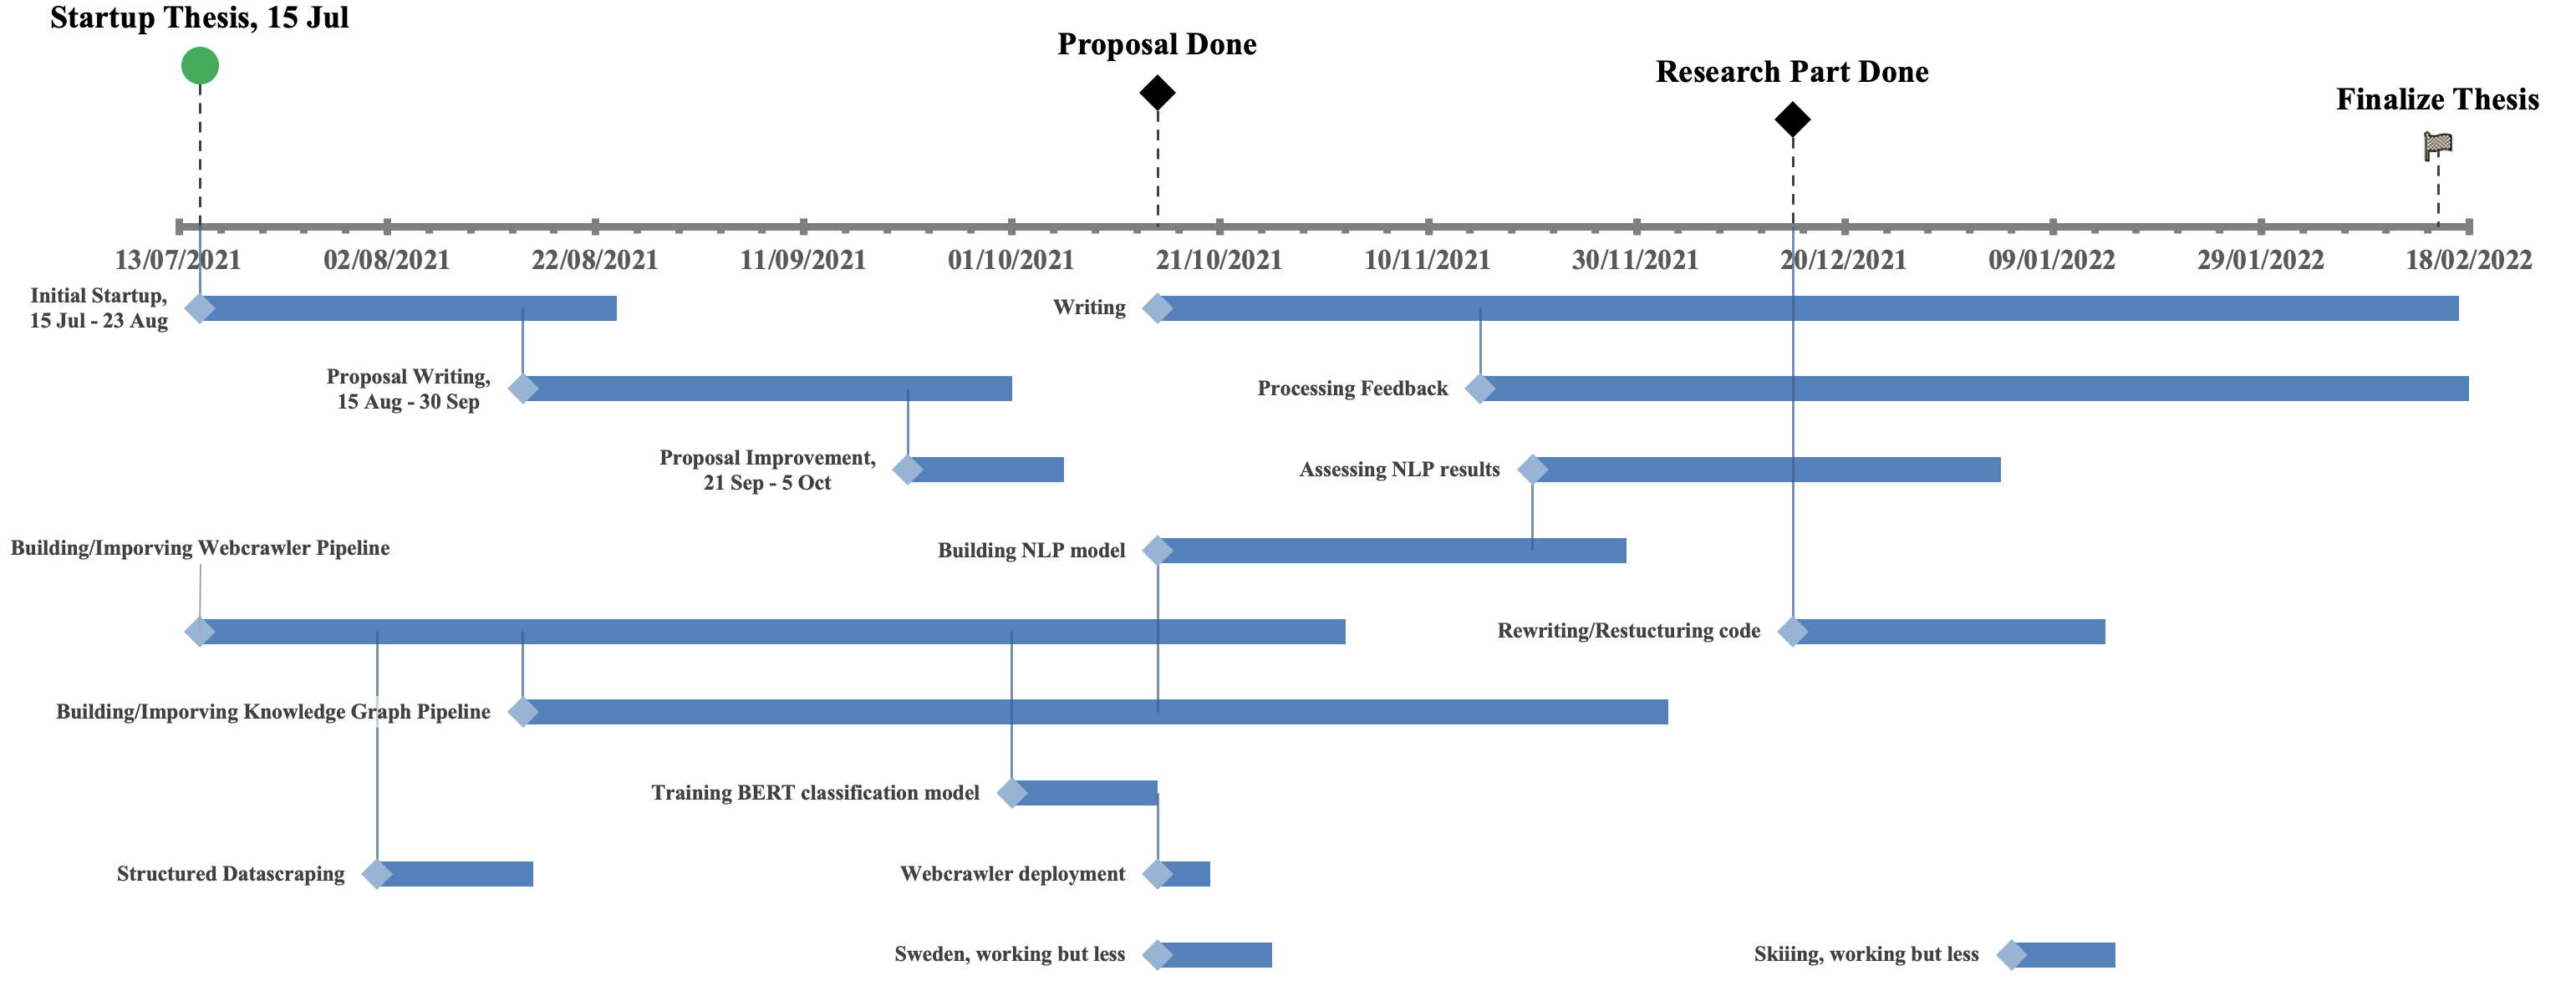
\includegraphics[width=1.6\textwidth]{schedule.png}}
    \caption{Time Schedule}
    \label{fig:time_schedule}
\end{figure}
%\end{landscape}
%\newpage

\section{Feasibility}
\newpage
\printbibliography
\end{document}


